\bchapter{NNAPI}
\section{Accelerazione Hardware}
La caratteristica principale dell’uso di NNAPI\cite{NNAPI} è l’accelerazione hardware. In particolare, uno smartphone è sicuramente dotato di una unità di elaborazione
centrale (CPU da ora in avanti), che esegue tutte le principali operazioni, sfruttando i registri, la cache, la ram ed eventuali storage. Grazie alla CPU
si possono svolgere tutte le operazioni di I/O, gestione memoria, grafica, gestione batteria, errori e quant’altro.
La CPU da sola, però, nella maggior parte dei casi non riesce a reggere quantità elevate di calcolo, in quanto si trova già occupata a svolgere operazioni
base date dall’OS (Android nel nostro caso, ma anche iOS per esempio) e varie operazioni di I/O e memory. Proprio per questa sua limitazione, nella grande
maggioranza degli smartphone moderni si trovano installati nella Motherboard anche altri componenti, in particolare una Scheda Video (GPU) ed eventualmente
altri moduli quali Digital Signal Processor (DSP) e Neural Processing Unit (NPU). 
Una scheda video, come suggerisce il nome, fornisce la potenza di calcolo necessaria a renderizzare ogni aspetto legato alla GUI dell’utente, ma non solo,
infatti grazie alla sua elevata potenza, può essere ampiamente sfruttata per tutte le operazioni che richiedono una grande quantità di dati da elaborare e
lo stesso può essere detto per DSP. 
Discorso a parte per le NPU. Si tratta di un processore “complementare” adatto a eseguire operazioni di calcolo prettamente incentrate sulle reti neurali.
Su ambienti mobile la prima comparsa è stata nel 2017, quindi relativamente recente, grazie alla presenza di una NPU sul chip kirin 970, presente nel Huawei
Mate 10 pro.
La sola integrazione di questo componente ha portato grandi vantaggi in termini di prestazioni e di efficienza energetica (si parla di un 50\% di efficienza
energetica guadagnata rispetto alla gamma precedente) rendendolo di fatto importante per tutti i prodotti successivi. Grazie a questa novità da parte di
Huawei anche i vari competitors iniziarono a produrre, ricercare e sperimentare il più possibile per stare al passo con il mercato, rendendo di fatto le NPU,
e il mondo dell’AI e delle reti neurali in generale, una realtà quotidiana presente su piccolo schermo.

Tornando quindi all’accelerazione hardware, il punto cardine è la possibilità di sfruttare tutti gli altri componenti oltre alla CPU per eseguire complesse
operazioni di calcolo e facilitare l’elaborazione di dati. 
In tema reti neurali, si ottiene un guadagno sotto più punti di vista per quanto riguarda operazioni di inferenza. Sicuramente si ottiene un incremento
nella velocità di risposta, in quanto il carico di lavoro viene efficientemente distribuito tra le varie unità di calcolo disponibili, e una ridotta
latenza generale, in quanto non c’è necessità di contattare un server esterno per richiedere dati.
Grazie a ciò non è nemmeno necessaria una connessione esterna, quale wifi o LTE, in quanto è possibile avere i dati in locale, rendendola di fatto
disponibile sempre e comunque in qualsiasi situazione a patto che ci sia batteria residua.
La questione energetica è un argomento piuttosto delicato, perché unità di elaborazione come GPU e DSP sono molto dispendiose in termini energetici e
spesso si deve ricorrere a compromessi.
Altro punto a sfavore, soprattutto per smartphone meno performanti, è la questione memoria. L’APK specifico potrebbe avere un peso di svariati GB e in
esecuzione la RAM potrebbe facilmente risultare piena, rischiando di portare il sistema in stati di rallentamenti o crash.
Un punto di forza è sicuramente la privacy, in quanto i dati rimangono all’interno del dispositivo.

\section{API Android Neural Networks}
L’API Android Neural Networks è una API pensata per eseguire operazioni pesanti, in termini di calcolo computazionale, per il machine learning su
dispositivi Android. In particolare la compatibilità SW è elevata, in quanto presente in ogni dispositivo con Android 8.1 (livello API 27) o successivo,
coprendo quindi più del 90\% dei dispositivi android attualmente in uso.

La NNAPI può essere sfruttata programmando in linguaggio C/C++ e sfruttando librerie di sistema di livello superiore come "Runtime NNAPI”.
Runtime NNAPI si tratta di una libreria condivisa tra un’app e i driver back-end con la particolarità di essere aggiornabile, per ricevere aggiornamenti
al di fuori del normale ciclo di rilascio di Android. Gli sviluppatori, quindi, possono correggere più facilmente bug presenti nel runtime e migliorarne
le compatibilità con i driver.

La vera potenza di queste API però, risiede nella possibilità di essere sfruttate da framework superiori come TensorFlow Lite, PyTorch o Caffe2 che
creano e addestrano reti neurali. Grazie a NNAPI è dunque possibile sfruttare modelli già definiti e allenati, avendo quindi un’abbondanza di dati a
disposizione.

\begin{figure}
    \centering
    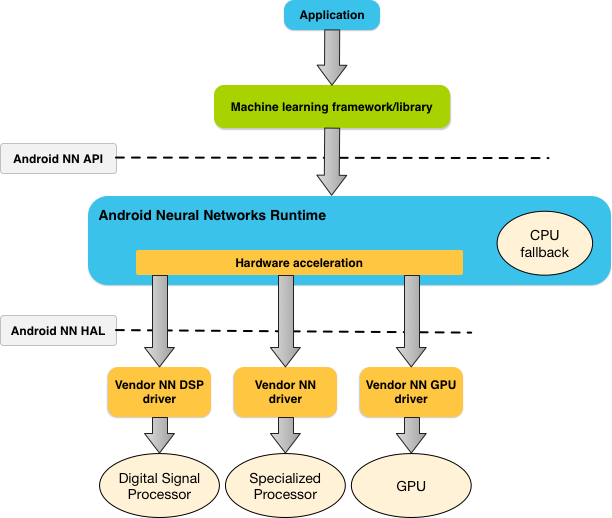
\includegraphics[width=0.8\textwidth]{Immagini/nnapi_architecture.png}
    \caption{Architettura di sistema per l'API Android Neural Networks.}
    \label{fig:nnapiArchitecture}
\end{figure}

In figura \ref{fig:nnapiArchitecture} si riesce a visualizzare facilmente il flusso di lavoro. L’applicazione utilizza le librerie e i framework di machine
learning (come PyTorch o Runtime NNAPI) che a loro volta sfruttano le API di basso livello di NNAPI.
NNAPI comunica con l’astrazione HW del dispositivo per rete neurale, contattando i driver che si interfacciano all’hardware specifico (GPU, DSP ecc.).
Questo meccanismo efficace permette di dividere il lavoro in vari livelli di astrazione, in modo da isolare i compiti e ridurre problematiche, aumentando
la rapidità di risoluzione dei vari bug presenti. Questo meccanismo di divisione dei compiti è alla base di due importanti design pattern, in particolare
“Responsibility”, che permette di dividere le responsabilità ad ogni layer, e “Layered Architecture”, che come suggerisce il nome è un pattern architetturale
che come concetto alla base ha la suddivisione del software in vari strati. La tipologia sopra descritta è alla base della progettazione Android e Java.

Per sfruttare i calcoli tramite NNAPI è necessario prima creare un grafico diretto che definisca i suddetti calcoli. Questo grafico infatti, combinato con
i vari dati di input, forma il modello per la valutazione del runtime NNAPI. Vengono definite 4 astrazioni principali con NNAPI:
\begin{itemize}
    \item \textbf{Modello}: si tratta di un grafico di calcolo delle operazioni matematiche e di tutti i valori costanti appresi durante il processo
    di addestramento e sono operazioni specifiche delle reti neurali. Includono convoluzione bidimensionale\footnote{https://en.wikipedia.org/wiki/Convolution}
    (2D), attivazione logistica (sigmoid\footnote{https://en.wikipedia.org/wiki/Sigmoid\_function}), attivazione lineare rettificata\footnote{https://en.wikipedia.org/wiki/Rectifier\_(neural\_networks)}
    (ReLU) e altro ancora. Una volta creato correttamente, può essere utilizzato nuovamente in tutti i vari thread e le compilation. In NNAPI, un modello
    è rappresentato come un'istanza ANeuralNetworksModel\footnote{https://developer.android.com/ndk/reference/group/neural-networks?hl=it\#aneuralnetworksmodel}.
    La creazione di un modello è un'operazione sincrona.
    \item \textbf{Compilation}: rappresenta una configurazione per compilare un modello NNAPI in codice di livello inferiore. La creazione di una
    compilazione è un'operazione sincrona. Una volta creato correttamente, può essere riutilizzato in più thread ed esecuzioni. In NNAPI, ogni
    compilazione è rappresentata come un'istanza ANeuralNetworksCompilation\footnote{https://developer.android.com/ndk/reference/group/neural-networks?hl=it\#aneuralnetworkscompilation}.
    \item \textbf{Memoria}: rappresenta la memoria condivisa, i file mappati di memoria e buffer di memoria simili. L'utilizzo di un buffer di memoria
    consente al runtime NNAPI di trasferire i dati ai driver in modo più efficiente. In genere, un'app crea un buffer di memoria condiviso contenente
    tutti i tensori necessari per definire un modello. Puoi anche utilizzare i buffer di memoria per archiviare gli input e gli output per un'istanza di
    esecuzione. In NNAPI, ogni buffer di memoria è rappresentato come un'istanza ANeuralNetworksMemory\footnote{https://developer.android.com/ndk/reference/group/neural-networks?hl=it\#aneuralnetworksmemory}.
    \item \textbf{Esecuzione}: interfaccia per l'applicazione di un modello NNAPI a un insieme di input e per la raccolta dei risultati. L'esecuzione
    può essere eseguita in modo sincrono o asincrono. Per l'esecuzione asincrona, più thread possono attendere la stessa esecuzione. Al termine di questa
    esecuzione, tutti i thread vengono rilasciati. In NNAPI, ogni esecuzione è rappresentata come un'istanza ANeuralNetworksExecution\footnote{https://developer.android.com/ndk/reference/group/neural-networks?hl=it\#aneuralnetworksexecution}.
\end{itemize}

\begin{figure}
    \centering
    \includegraphics[width=0.9\textwidth]{Immagini/nnapi\_flow.png}
    \caption{Flusso di programmazione per l'API Android Neural Networks.}
    \label{}
\end{figure}

\section{Modello}
L'unità di calcolo fondamentale in NNAPI è il modello, il quale è definito da uno o più operandi e operazioni.
Gli operandi sono oggetti di dati utilizzati nella definizione del grafico, tra i quali costanti, input e output e nodi intermedi e possono essere di due tipi: scalari e tensori.
Uno scalare è un singolo valore nei vari formati booleano, interi, virgola mobile a 16, 32 bit.
I tensori, invece, sono array n-dimensionali. In NNAPI i tensori possono anche essere quantizzati a 8 o 16 bit.

\begin{figure}[ht]
    \centering
    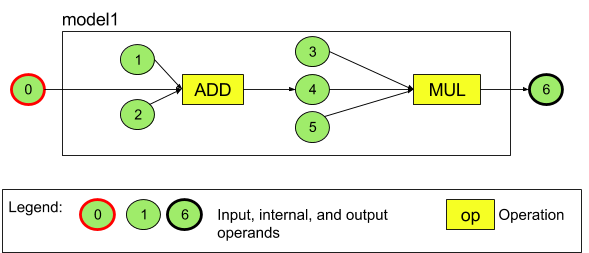
\includegraphics[width=0.7\textwidth]{Immagini/operandi.png}
    \caption{Esempio di operandi per un modello NNAPI}
    \label{fig:operandi}    
\end{figure}

\subsection{Fasi operative}
In NNAPI, un'operazione specifica i calcoli da eseguire, costituita dai seguenti elementi:
\begin{itemize}
    \item un tipo di operazione (ad es. addizione, moltiplicazione, convoluzione);
    \item un elenco di indici degli operandi utilizzati dall'operazione per l'input;
    \item un elenco di indici degli operandi utilizzati dall'operazione per l'output.
\end{itemize}
Prima di aggiungere l'operazione, devi aggiungere al modello gli operandi utilizzati o prodotti da un'operazione.

L’utilizzo delle Neural Networks API avviene a basso livello, grazie a linguaggi come C/C++. In particolare C++ rispecchia la programmazione ad oggetti (come lo sono Java e Kotlin) e permette quindi di
definire veri e propri modelli come oggi in maniera intuitiva.
Per creare un modello, per esempio, basta definire due righe di codice:
\begin{center}
\texttt{ANeuralNetworksModel\* model = NULL;} \\ \texttt{ANeuralNetworksModel\_create(\&model);}\\
\end{center}
Dopo la creazione è necessario aggiungere i vari operandi attraverso \texttt{ANeuralNetworks\_addOperand()} e sfruttando le strutture dati fornite, come \textit{ANeuralNetworksOperandType}.

\section{Compilation}
In questa fase viene determinato su quali processori verrà eseguito il modello e chiede ai driver corrispondenti di preparare l’esecuzione, anche eventualmente generando codice macchina specifico per i processori scelti.
Da sottolineare la possibilità di scegliere esplicitamente quali dispositivi utilizzare e il rapporto di runtime tra l’utilizzo della batteria e la velocità di esecuzione.

\subsection{Esecuzione Sincrona VS Asincrona}
Alcune operazioni nel runtime NNAPI sono eseguite in maniera sincrona. Ciò significa che ogni operazione di questo tipo può rallentarne l’esecuzione, in quanto è necessario attendere la fine di un’esecuzione per iniziare
la successiva e viene ridotta la potenza innata del multithreading.

Di contro, sfruttare esecuzioni asincrone non sempre è conveniente, in quanto il dispositivo deve poter generare e sincronizzare tutti i vari thread, con latenza variabile. A volte è possibile avere ritardi di più di
500 microsecondi tra quando viene inviata la notifica di un thread al momento in cui viene associato un core. 

Da Android 10 in poi, NNAPI supporta esecuzioni di burst tramite un oggetto apposito. Le esecuzioni burst altro non sono che sequenze di esecuzioni della stessa compilazione che si verificano in rapida successione,
come la campionatura audio o l’acquisizione video. Gli oggetti burst quindi può portare ad esecuzioni più rapide, dove gli acceleratori rimangono in uno stato di prestazioni elevate per tutta la durata burst.

\subsection{Gestione errori}
Di norma, se si verifica un errore durante il partizionamento o un errore con i driver scelti, NNAPI ricorre alla implementazione della CPU per una o più operazioni ove possibile. Sfruttando framework come TensorFlow Lite
nella maggior parte dei casi può essere vantaggioso disabilitare la riserva della CPU e gestire gli errori con implementazioni delle operazioni ottimizzate dal client.

Se il partizionamento o la compilazione non vanno a buon fine, l’intero modello sarà provato sulla CPU, stessa cosa vale per un’operazione che continua a non riuscire. Questo ovviamente riduce notevolmente la velocità
di esecuzione ma aumenta le possibilità di successo, riducendo eventuali errori hardware. Da considerare, però, che alcune operazioni non sono nemmeno supportate dalla CPU.

È possibile quindi disabilitare il fallback della CPU e rimuoverla dall’elenco dei processori nel caso in cui non la si voglia utilizzare per operazioni del modello.

\subsection{Memoria}
Da sottolineare la possibilità, da Android 11 e successive, di sfruttare domini di memoria che forniscono interfacce allocatrici per memorie opache. Ciò permette alle applicazioni di passare dati e ricordi nativi del
dispositivo tra le varie esecuzioni, in modo che NNAPI non copi o trasformi i dati inutilmente quando eseguono esecuzioni consecutive sullo stesso driver.

Queste funzionalità sono destinate principalmente ai tensori interni ai driver con pochi accessi lato client, come tensori di stato. Per tensori con frequenti accessi alla CPU lato client, è necessario utilizzare pool di memoria condivisi.

\section{Tempo di esecuzione}
Il test delle prestazioni di un'app può essere effettuato misurando il tempo di esecuzione o tramite profilazione. Per misurare il tempo di esecuzione, si può utilizzare l'API di esecuzione sincrona o API a livello inferiore
come ANeuralNetworksExecution\_setMeasureTiming e ANeuralNetworksExecution\_getDuration. Queste API consentono di misurare il tempo di esecuzione su un acceleratore o nel driver, escludendo l'overhead come quello del runtime NNAPI
e dell'IPC.

Le informazioni di tempistica possono essere utili per ottimizzare le prestazioni dell'applicazione in produzione, anche se la raccolta di tali informazioni potrebbe influenzare le prestazioni stesse, da notarne in fase di
controllo e revisione dei dati. È importante notare che solo il driver è in grado di calcolare il tempo trascorso su se stesso o sull'acceleratore.
Per profilare l'applicazione, si può utilizzare Android Systrace, che genera automaticamente eventi systrace per profilare diverse fasi del ciclo di vita del modello e i vari livelli dell'applicazione, come Application,
Runtime, IPC e Driver.

Per generare i dati di profilazione NNAPI, è possibile utilizzare il comando systrace di Android e l'utilità parse\_systrace. Questi strumenti consentono di analizzare gli eventi systrace generati dall'applicazione e di ottenere
una visualizzazione tabellare dei tempi spesi nelle diverse fasi del ciclo di vita del modello e nei diversi livelli dell'applicazione.
Inoltre, Android 11 introduce miglioramenti nella qualità del servizio (QoS) per NNAPI, consentendo alle applicazioni di indicare le priorità relative dei propri modelli e di impostare timeout per la compilazione e l'inferenza del modello.

Infine, sono disponibili argomenti avanzati sull'utilizzo degli operandi NNAPI, come tensori quantizzati, operatori facoltativi e tensori di ranking sconosciuto. Il benchmark NNAPI è disponibile su AOSP per valutare latenza e accuratezza
dei modelli.

\subsection{Log}
NNAPI offre informazioni diagnostiche utili nei log di sistema, che possono essere analizzati utilizzando l'utilità logcat. È possibile attivare il logging dettagliato per fasi o componenti specifici impostando la proprietà
\textit{debug.nn.vlog} tramite adb shell. Questo consente di registrare informazioni dettagliate su fasi come la creazione di modelli, la compilazione, l'esecuzione e altro ancora.

Una volta attivato, il logging dettagliato genererà voci di log a livello di informazioni con un tag impostato sul nome della fase o del componente. Per controllare il livello dei messaggi di log mostrati da logcat si utilizza
la variabile di ambiente \textit{ANDROID\_LOG\_TAGS}. Questo è solo un filtro applicato a logcat e si deve comunque impostare la proprietà debug.nn.vlog su all per generare informazioni di log dettagliate



